%Die Angabe des schlauen Spruchs auf diesem Wege funtioniert nur,
%wenn keine Änderung des Kapitels mittels den in preambel/chapterheads.tex
%vorgeschlagenen Möglichkeiten durchgeführt wurde.
\chapter{Experimental Setup}
\label{chap:chapter5}
%\vspace{-3cm}
%\vspace{2cm}
With the selection and their extraction and SVM, as the selected machine learning algorithm explained in earlier chapter, this chapter explains the experimental setup. This chapter focuses on two topics - first part being the assumptions for the test setup and the configuration of the sample population as well as the method used to generate the sample population, explained in the section~\ref{sec:gsp}. Second part, section~\ref{sec:libsvm} describes the SVM library used for training and classification of faults and its interface with generated samplae population.
\section{Generation of sample population}
\label{sec:gsp}
Sample population is required to train and cross-validate the machine learning based classifier (hereon referred simply as \emph{classifier}). A separate set of data is used to test the accuracy of the classifier.
\subsection{Assumptions}
\label{sec:gsp:assumptions}
Following are the assumptions while generating the sample population and test data:
\begin{enumerate}
  \item It is assumed that the chips to be classified have displayed faulty behavior and hence were rejected in earlier test.
  \item The chips under consideration are either:
		  \begin{enumerate}
    		\item Healthy chips with transient noise or
    		\item Affected by a single permanent or intermittent fault, with or without transient noise.
 		 \end{enumerate}
	\item Number of simulation runs to extract features is fixed at 4. This value is set experimentally. 
\end{enumerate}

\subsection{Configuration}
\label{sec:gsp:configuration}
For the purpose of running experiments uniformly on different circuit types, a sample population and a test set for each of circuit types is created with following configuration:
\begin{enumerate}
  \item A sample population consist of 2500 ($\pm$ 75) of labeled examples. The tolerance of $\pm$ 75 is set as the permanent or intermittent fault instances which did not show any faulty behavior at POs at all were removed.
  \item The sample population is equally divided into following five fault categories:
		\begin{enumerate}
    		\item Permanent faults with label \texttt{P}.
    		\item Permanent faults along with transient noise (fault rate = 0.001) with label \texttt{P}.
			\item Intermittent faults (fault rate = 0.1, 0.01 0.001) with label \texttt{I}.
    		\item Intermittent faults (fault rate = 0.1, 0.01, 0.001) along with transient noise (fault rate = 0.001) with label \texttt{I}.
			\item Transient faults (fault rate = 0.01, 0.001, 0.0001) with label \texttt{T}.
		\item Permanent faults are modeled using stuck-at, wired or delay faults, Intemittents are modeled using high frequency power droop, and transient faults are modeled as conditional stuck-at faults at random locations, triggered using deterministic fault rate.
 		 \end{enumerate}
  \item Test data has 250 ($\pm$ 15) labeled examples, with same configuration as that for sample population.
\end{enumerate}

\subsection{Implementation}

Sample population is generated as shown in figure~\ref{fig:sampopl} using a simulation framework called Adaptive Diagnosis of Arbitrary Manifold Artifacts (ADAMA). ADAMA can be used for logic simulation with error injection. Logical representation of a circuit at gate level and test pattern set are the required inputs for simulation using ADAMA. A fault description can be provided optionally to inject a fault and analyze its behavior. ADAMA supports all of the fault models that have been considered under configuration in section~\ref{sec:gsp:configuration}.

\begin{figure}[h]
  \begin{center}
    \captionsetup{justification=centering}
    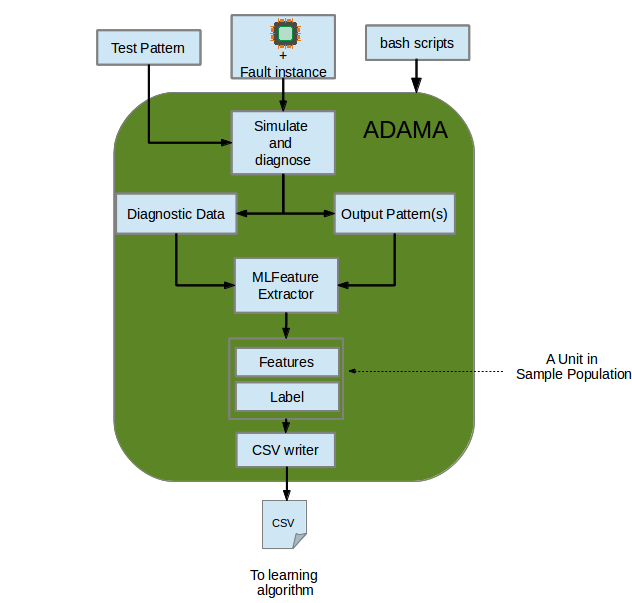
\includegraphics[scale=0.45]{figures/sampopl.png}
    \caption{Generation of sample population using \texttt{spgen}}
    \label{fig:sampopl}
  \end{center}
\end{figure}

For experiments, ADAMA framework has been extended by adding a task to generate sample population, called \texttt{spgen}.\texttt{spgen} takes fault description, circuit description and test pattern set as inputs along with number of simulations runs (\texttt{simruns}) to be performed for feature extraction. It then runs simulation and diagnosis \texttt{simruns} times and passes it on to the object of class \texttt{MLFeatureExtractor}, which encompasses all of the procedures for feature extraction described in section~\ref{sec:secfs} of previous chapter. Once complete simulation is over, it writes the features and its label in a CSV file.

Shell scripts are used to invoke instances of ADAMA and inject fault instances of permanent, transient and intermittent faults. The process to do the same is described below:

\begin{description}
  \item[Permanent Faults] A task in ADAMA called \texttt{fsample} is used to generate fault descriptions for permanent faults. Script first runs task \texttt{fsample} and puts all fault descriptions in a file, and then parses it line-by-line to invoke an instance of ADAMA with task \texttt{spgen}. It then uses same fault descriptions and adds a transient fault instance to generate transient noise and runs the complete process again, while logging seed values used to generate transients. After generation of features is done, it scans through the feature file of permanent faults without transient noise and scans for fault instances which did not result in failure at POs and removes corresponding features, fault descriptions and corresponding items in feature file for permanent faults with transient noise.

  \item[Intermittent faults] Script first generates intermittent fault descriptions with random seed values for location and fault activation and store them into a file. It then invokes \texttt{spgen} using ADAMA and simulates these fault instances first without and then with transient noise, while logging all seed values and corresponding fault rates. The fault descriptions and and corresponding examples in feature files of intermittent faults and intermittent faults with transient noise are removed, where intermittent fault as not active at least for one simulation round.

  \item[Transient faults] Script takes circuit description and passes it, along with a transient fault instance with defined fault rate and a randomly generated seed value to \texttt{spgen} in ADAMA. It also logs seed values and corresponding fault rates used for generation of transient fault instances.
\end{description}

\section{Library for SVM based classification - \texttt{LIBSVM}}
\label{sec:libsvm}
\texttt{LIBSVM} \cite{Chang2011} is a popular SVM library, used in variety of applications. It supports linear, polynomial, radial and sigmoid kernel functions and also supports custom user kernels. For experiments, all of the available kernels in the tool have been used, to find out accuracy levels for each of them. It is coded in C++ and Java and it is available as open-source software available for free use under modified BSD license. It supports multi-class classification using multiple binary classifiers. \texttt{LIBSVM} comes with scripts to train the tool and to find optimal parameters for classification.

\subsection{Training}

\begin{figure}[h]
  \begin{center}
    \captionsetup{justification=centering}
    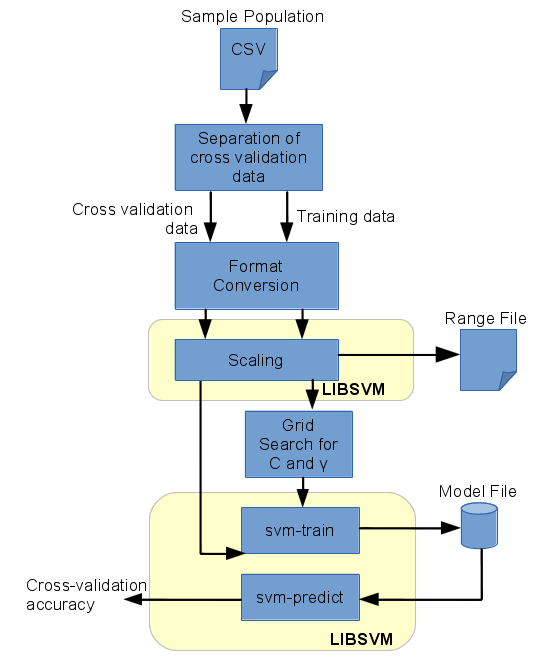
\includegraphics[scale=0.75]{figures/libsvmtrain.png}
    \caption{Steps to train SVM using \texttt{LIBSVM}}
    \label{fig:libsvmtrain}
  \end{center}
\end{figure}

Sequence of steps followed to train SVM, as shown in figure~\ref{fig:libsvmtrain} is as follows:
\begin{description}
   \item[Format conversion] \texttt{LIBSVM} requires input in \emph{sparse} format. A utility function \texttt{convert} provided by authors of \texttt{LIBSVM} has been extended to be compatible with the CSV format output of \texttt{spgen}.

  \item[Scaling] \texttt{svm-scale} executable file in \texttt{LIBSVM} provides functionallity to scale the training data to user specified input range. Documentation of \texttt{LIBSVM} \cite{Hsu2003} suggest use of range [0,1] for the data containing zero values for some of feaures, as in our case. The scaling parameters are stored in a \emph{range file}, which is later used to scale features of future examples or test data.
  
  \item[Grid search for C and $\gamma$] \texttt{LIBSVM} provides a script to find suitable values of C and $\gamma$. The grid search algorithm uses $v$-fold cross-validation (CV), meaning that the data is divided into $v$ subsets and one subset is tested against classifier trained with rest of $v-1$ subsets, iteratively until complete training set is covered \cite{Hsu2003}.  This results in the training data being tested once completely, and corresponding accuracy is called as \emph{cross-validation accuracy}. The algorithm then tries various pairs of C and $\gamma$ to find a pair with the highest CV accuracy. This script internally uses \texttt{svm-train} for modeling classifiers, when it calculates CV accuracy, hence the kernel type for training needs to be specified. This script was extended to take kernel type as input.
 
 \item[Training] \texttt{svm-train} executable file in \texttt{LIBSVM} is used for training SVM. It tries to solve the minimization problem (refer section~\ref{mltypes:svm}) to find out best fitting model for the SVM. Kernel to be used for training needs to be provided as input at this stage also. It outputs a \emph{model file} to be used for prediction of future examples.
\end{description}

\subsection{Classification}

Steps to classify data using already trained SVM is shown in figure~\ref{fig:libsvmpredict}. A short description of the these is noted below:

\begin{figure}[h]
  \begin{center}
    \captionsetup{justification=centering}
    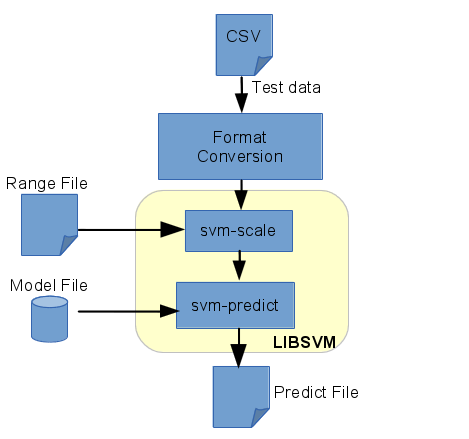
\includegraphics[scale=0.75]{figures/libsvmpredict.png}
    \caption{Steps for classification of test data with SVM using \texttt{LIBSVM}}
    \label{fig:libsvmpredict}
  \end{center}
\end{figure}

\begin{description}

   \item[Format conversion] Using the same tool used for format conversion of training data, format of test data is also converted to sparse format.

  \item[Scaling] The test data is scaled using \texttt{svm-scale}. The range file generated while scaling the training data is used in this step to scale the test data.
  
  \item[Prediction] \texttt{svm-predict} tool provided with \texttt{LIBSVM} is used to predict the test data. \texttt{svm-predict} needs model file generated during training as input and it outputs \emph{predict file} with predicated labels of the test data. This file is further processed using scripts for evaluation of accuracy levels of different fault classes.
  
\end{description}
